\documentclass{article}
\usepackage{amsmath}
\usepackage{caption}

\def\apeqA{\SavedStyle\sim}
\def\apeq{\setstackgap{L}{\dimexpr.5pt+1.5\LMpt}\ensurestackMath{%
      \ThisStyle{\mathrel{\Centerstack{{\apeqA} {\apeqA} {\apeqA}}}}}}

% if you need to pass options to natbib, use, e.g.:
% \PassOptionsToPackage{numbers, compress}{natbib}
% before loading nips_2017
%
% to avoid loading the natbib package, add option nonatbib:
% \usepackage[nonatbib]{nips_2017}

\usepackage[final]{nips_2017}

\usepackage{graphicx}
\usepackage[utf8]{inputenc} % allow utf-8 input
\usepackage[T1]{fontenc}    % use 8-bit T1 fonts
\usepackage{hyperref}       % hyperlinks
\usepackage{url}            % simple URL typesetting
\usepackage{booktabs}       % professional-quality tables
\usepackage{amsfonts}       % blackboard math symbols
\usepackage{nicefrac}       % compact symbols for 1/2, etc.
\usepackage{microtype}      % microtypography

\newcommand{\lstm}{LSTM }

% Choose a title for your submission
\title{Project 2: Predicting the End of a Story}


\author{Student 1 \qquad Student 2 \qquad Student 3}

\begin{document}
% \nipsfinalcopy is no longer used

\maketitle

% We do not requrire you to write an abstract. Still, if you feel like it, please do so.
%\begin{abstract}
%\end{abstract}

%Feel free to add more sections but those listed here are strongly recommended.

\section{Introduction}
\label{sec:intro}

Natural language is
You can keep this short. Ideally you introduce the task already in a way that highlights the difficulties  your method will tackle.

\section{Methodology}
The idea of our approach follows that of successes in previous work such as \cite{UWNLP}, \cite{Goel} and \cite{COGCOMP}. More specifically our approach consists of training a binary logistic regression classifier based on an augmented data set which we create ourselves. This augmentation is based on ideas that have been successfully used in the past (e.g. \cite{LSTMClassifier}\cite{SENTENCE_EMB}). As features for our classifier we consider a collection of feature extractors which produce a vector of features for any 5 sentence story.

\subsection{Data augmentation}
The augmented data set is composed of labeled 5 sentence stories. We create it by combining the original ROCStory corpus intoduced by \cite{ROCstories} and a negative data set. Here the ROC dataset gets assigned a positive label and the negative set a negative label. We compose the negative dataset by replacing the ending of each 5 sentence story by a randomly selected ending, as done by \cite{LSTMClassifier}. Throughout this paper we use a replication factor of 1 i.e. for every sample of the original training set we add a single negative sample.

\subsection{Feature extraction}
In order to fit a logistic regression model as described above we use features obtained from feature extractors. A feature extractor is simply a model which takes in a 5 sentence story and outputs a feature or vector of features. Feature extractors are discussed extensively in section 3. To obtain the final set of features we simply combine features from all extractors for each sample.

\subsection{Classification}
After extracting features we fit a classifier to be able to distinguish between a fake (negative) story and a true (positive) one.
%Your idea. You can rename this section if you like. Early on in this section -- but not necessarily first -- make clear what category your method falls into: Is it generative? Discriminative? Is there a particular additional data source you want to use?

\section{Model}

	\begin{figure}[h!]
		\centering
		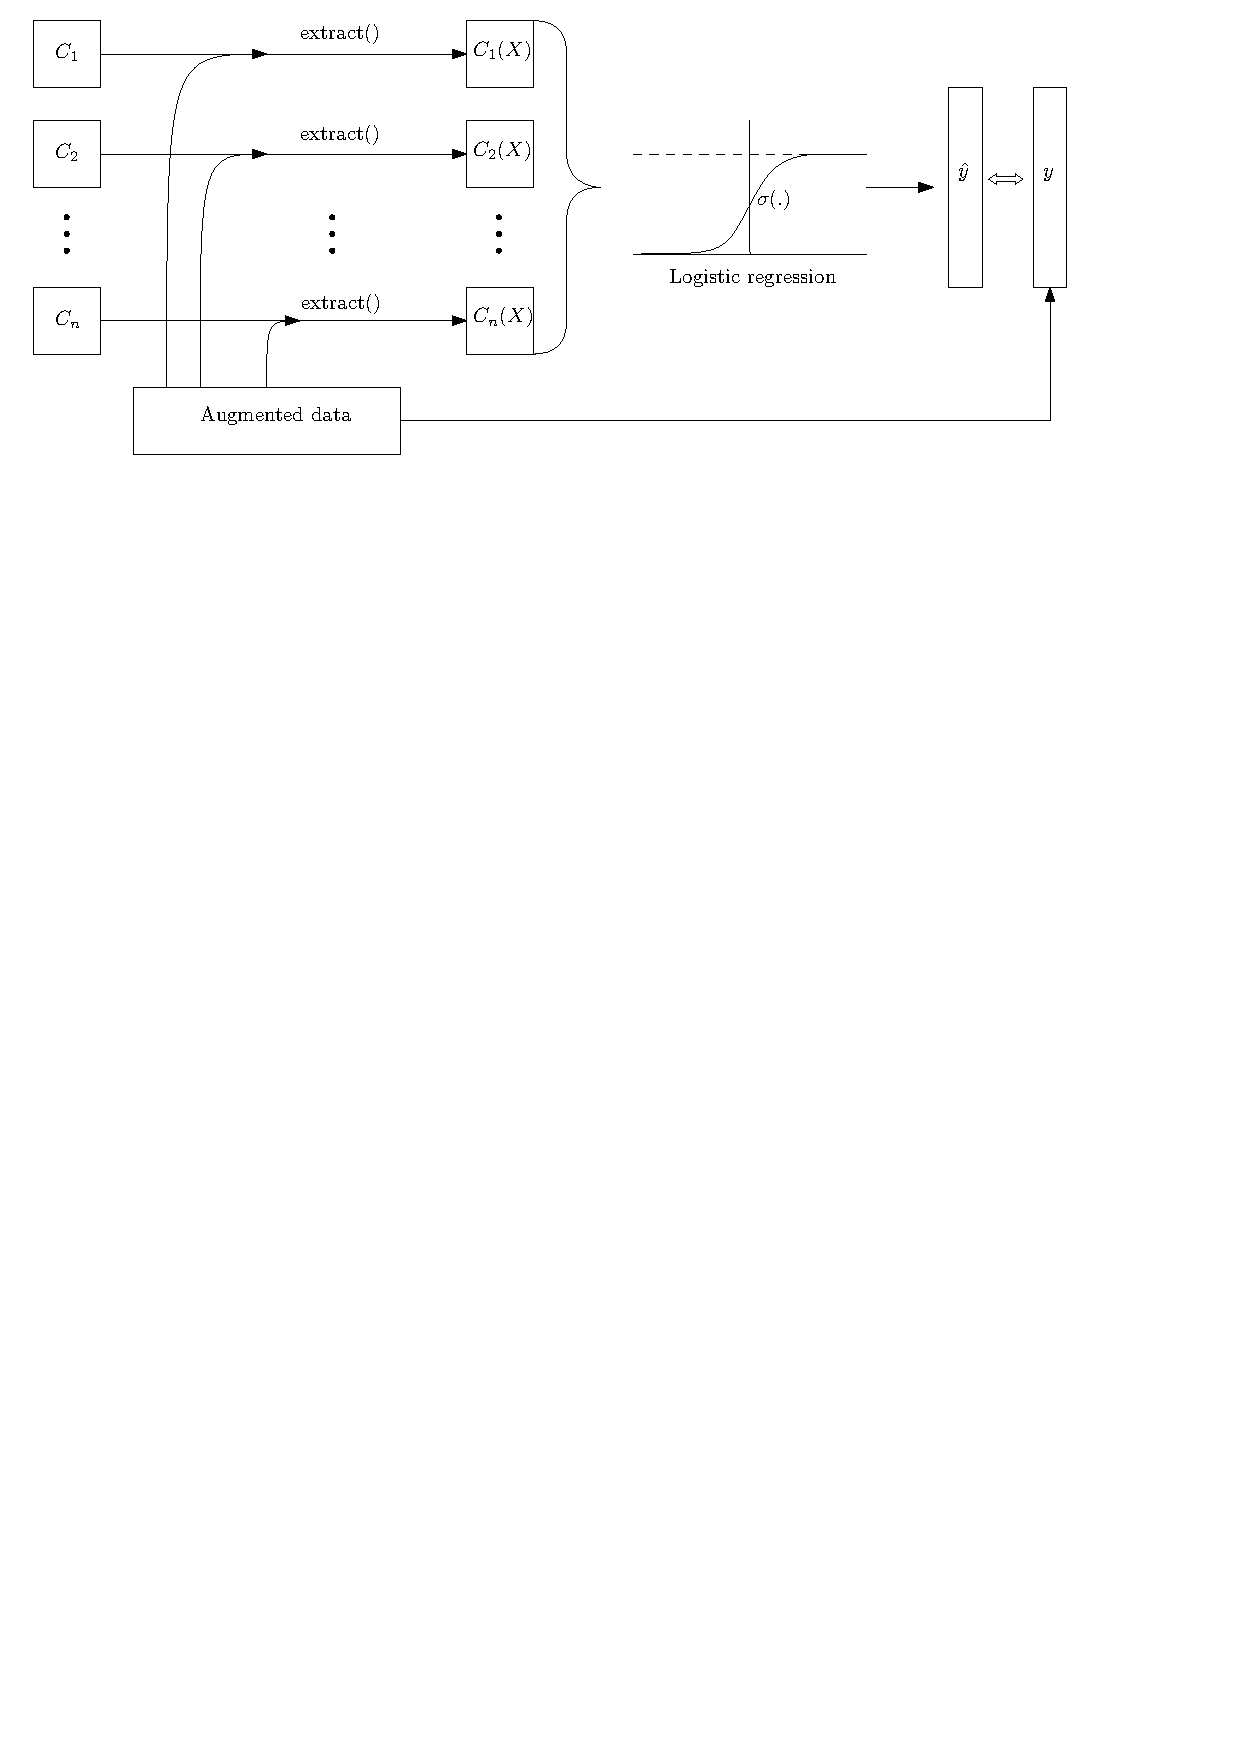
\includegraphics[scale=0.8]{fig/logistic_fitting.pdf}
		\caption{Main components of the global approach.}
		\label{Main}
	\end{figure}

The core components of our approach can be seen in figure \ref*{Main}. As described in section 2.2, the $C_i$ are the feature extractors and indicates a mapping:
\begin{equation}
C: \mathbb{S}^5 \rightarrow \mathbb{R}^l
\end{equation}
That is, afunction of the set of all 5 sentence stories ($\mathbb{S}^5$) to a real vector. We apply all the feature extractions to the augmented dataset as described in section 2.1. This is denoted by $C_i(X)$ in figure \ref*{Main}. We then apply logistic regression implemented in scikit-learn \cite{SKL} using the extracted dataset and the labels of the augmented set.

\pagebreak
\subsection{Fitting extractors}
In order to extract features from 5 sentence stories, the extractors have to be fitted first. This means it sees either an augmented data set or the original ROC data set. Figure \ref*{fit} shows the general approach for fitting extractors.
%\begin{figure}[h!]
%	\centering
%	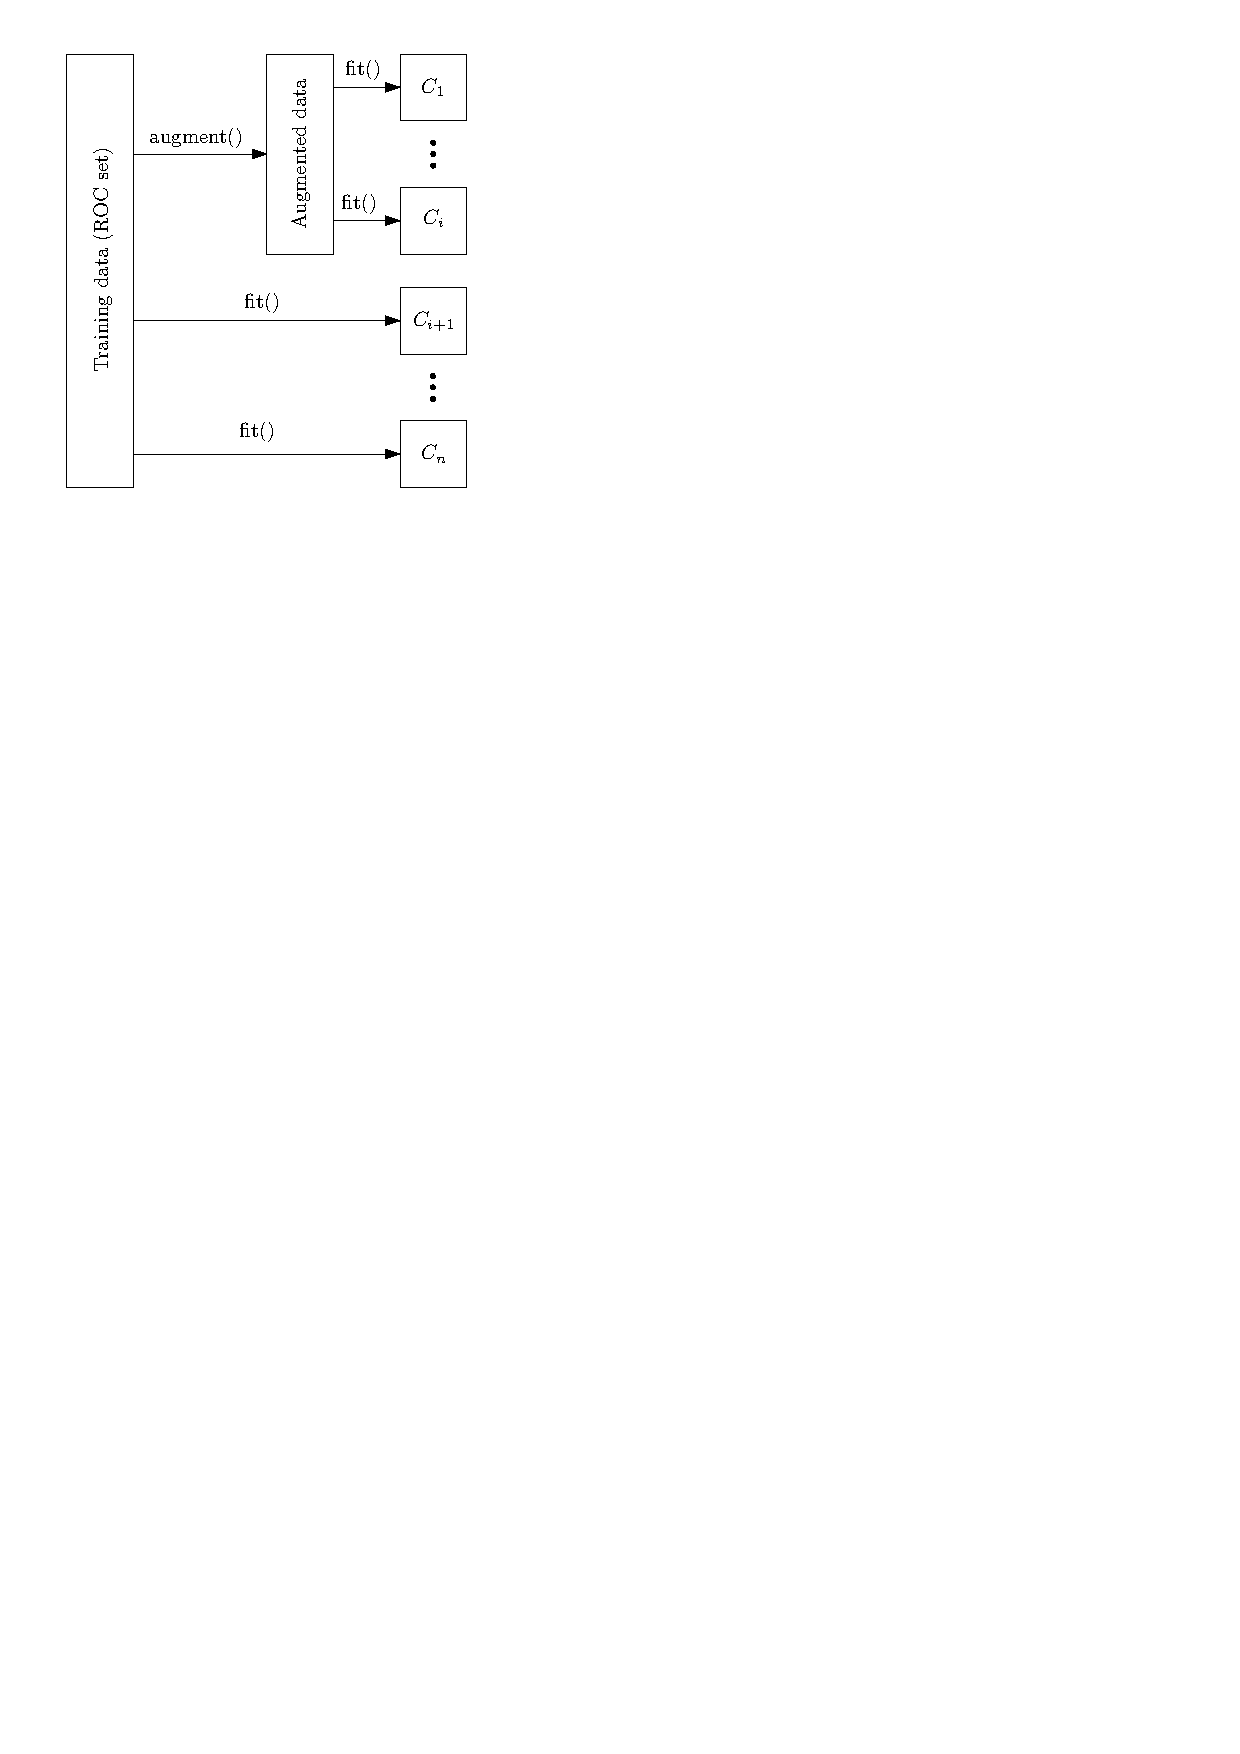
\includegraphics[scale=0.8]{fig/extractors_fitting.pdf}
%	\caption{Fitting feature extractors by using the Original ROC set or the augmented set.}
%	\label{fit}
%\end{figure}

\subsection{Different extractors}
This subsection we discuss various feature extraction methods we implemented in the model in extensive detail.\\\\
\textbf{Sentiment trajectory} This feature was previously explored by \cite{COGCOMP} and is based in the fact that stories often follow a certain emotional path. e.g. a story with a positive introduction might have a sad climax but a happy ending. In this feature we consider a story to be built as follows: the first sentence forms the introduction ($1$), the second and third form the body ($2$), the fourth forms the climax ($3$) and fifth forms the ending ($4$)\footnote{We have explored multiple ways of categorising the sentences in blocks and found this configuration to be the most effective, which is in allignment with \cite{COGCOMP}.}.To model this trajectory we considered the following distribution:
\begin{equation}
P(S_1,S_2,S_3,S_4)
\end{equation}
Where $S_i$ is the sentiment of the $i$'th block as defined above.
%The math/architecture of your model. This should formally describe your idea from above. If you really want to, you can merge the two sections.

\section{Training}
\label{sec:training}
%What is your objective? How do you optimize it?

In this section, we describe the results for the different extractors we apply
to the {\it Story Cloze task} as well as for our Ensemble method. For all our
approaches, the training set is first augmented as previously explained and then
used to train each of our extractors.

Table \ref{tab:params} shows the number of trainable parameters of the models we
used for the task and additionally the training duration. Our models were
trained using 15\% of the entire training data as validation data for training.
The accuracy with the actual validation set is evaluated after training is
completed. 

\begin{table}
    \caption{Training parameters.}
    \begin{center}
        \label{tab:params}
        \begin{tabular}{||c c c||} 
            \hline
            Method                 & \# Trainable parameters   & Training \\ [0.5ex] 
            \hline\hline
            Sentiment trajectory   & 80                        & $ \approx $ 45 secs. \\ 
            \hline
            Embedded closeness     & 0                         & $ \approx $ 5 secs.  \\
            \hline
            LSTM classifier        & $ \approx $ 200K          & 20 epochs \\ %$ \approx $ 1.2 hours \\
            \hline
            Language model         & $ \approx $ 1M            & 20 epochs \\ %$ \approx $ 20 hours \\
            \hline
            \textbf{Ensemble}      & 80                        & $ \approx $ 45 secs.  \\ [1ex] 
            \hline
        \end{tabular}
    \end{center}
\end{table}

The \lstm classifier was trained for 20 epochs using 15\% of the entire training
data as validation data for training. We did not perform more training epochs
due to the fact that we observed a decrease in the validation accuracy and an
increase of the loss function, i.e., the model was overfitting.  The language
model was trained for 20 epochs using a similar configuration as the \lstm
classifier. We observed that the loss function was still improving with the
number of epochs done. The sentiment trajectory method is based on using a
random forest classifier, thus its training phase is similar to other
classification methods and in this case is not time consuming.

\section{Results}
\label{sec:results}

Table \ref{tab:results} shows the accuracy obtained by different methods on the
validation and the provided test set. 

\begin{table}
    \caption{Accuracy on different data sets.}
    \begin{center}
        \label{tab:results}
        \begin{tabular}{||c c c||} 
            \hline
            Method                 & \# Validation set         & Test set \\ [0.5ex] 
            \hline\hline
            Sentiment trajectory   & 61.2\%                    & \textbf{60.4\%} \\ 
            \hline
            Embedded closeness     & 56.5\%                    & 55.4\% \\
            \hline
            LSTM classifier        & 51.4\%                    & 51.3\% \\ 
            \hline
            Language model         & 51.2\%                    & 50.02\% \\ [1ex] 
            \hline
        \end{tabular}
    \end{center}
\end{table}

Our approaches based on neural models were not able to perform as expected on
this task. For example, the \lstm classifier scored really high while training
(around 80\% accuracy). However it was not table to perform so well for the
task. This is because the model is able to capture sentences with the same
content, i.e., sentences containing the same subject, similar verbs and so on,
but not all stories contain the same subjects and verbs. Many times the stories
have a twist that our model is not able to capture although it might be obvious
for a human. Moreover, our language model was not able to go beyond a 50\%
accuracy on the test set. 

On the other hand, the sentiment trajectory model is able to capture the how the
story is actually evolving along the sentences. Thus, with this method we were
able to score a high accuracy on both data sets.

%This {\bf must} at least include the accuracy of your method on the validation set.

\section{Conclusion}
You can keep this short, too. \cite{*}

\bibliographystyle{plain}
\bibliography{bib/refs}
\end{document}
